\documentclass{article}
\usepackage[utf8]{inputenc}
\usepackage{amssymb}
\usepackage{amsmath}
\usepackage{cancel}
\usepackage{multirow}
\usepackage{graphicx}
\usepackage{forest}
\usepackage{algpseudocode}
\usepackage{algorithm}


\title{INFORMATICA TEORICA}
\author{giosumarin}
\date{March 2021}

\begin{document}

\maketitle

\tableofcontents


\section{Lezione 1}
\subsection{Definizione di funzione}

Funzione: una legge/regola che ci dice come associare un elemento di $A$ a uno di $B$.


\noindent
Definizione globale: $f:A\rightarrow B$: chiamiamo $A$ il dominio della funzione e $B$ il codominio.


\noindent
Definizione locale: $a\rightarrow^f b$ oppure $f(a)=b$ con $b$ immagine di $a$ rispetto a $f$ e $a$ controimmagine di $b$ rispetto a $f$. 


\noindent
$f:\mathbb{N} \rightarrow \mathbb{N}$ con $\mathbb{N}=\{0,1,2,3,4,..\}$ e con $\mathbb{N}^+=\{1,2,3,4,..\}$
\\
Globale: $f(n)=\lfloor \sqrt{n} \rfloor$; Locale: $f(5)=\lfloor \sqrt{n} \rfloor$
In una funzione, per definizione, un valore del dominio può portare a uno solo valore di codominio.

\subsection{Funzione iniettiva, suriettiva e biettiva}
\paragraph{Funzione Iniettiva}
\begin{displaymath}\label{iniettiva}
f:A\rightarrow B \textbf{ è iniettiva sse } \forall a_1, a_2 \in A \Rightarrow f(a_1) \neq f(a_2)
\end{displaymath}
ovvero non ci sono confluenze verso un punto del codominio.

\paragraph{Funzione Suriettiva}
\begin{displaymath}\label{suriettiva}
f:A\rightarrow B \textbf{ è suriettiva sse } \forall b \in B,  \exists a \in A: f(a)=b
\end{displaymath}

Definiamo con $Im_f$ l'insieme delle immagini. Quindi 
\begin{displaymath}\label{insieme_immagine}
    \{Im_f=b \in B: \exists a t.c. f(a)=b\}=\{f(a), a \in A\}
\end{displaymath}Possiamo quindi dire che in generale $Im_f \subseteq B$ ed è suriettiva sse $Im_f = B$, ovvero quando il grafico della funzione compre tutto l'asse $y$.

\paragraph{Funzione Biettiva}
Una funzione si dice biettiva quando è sia iniettiva che suriettiva, ovvero
\begin{displaymath}\label{biettiva}
    \forall b \in B \exists ! a \in A: f(a)=b
\end{displaymath}
dove con $\exists!$ indichiamo "esiste unico".

\paragraph{Composizione di funzioni}
Nota: non è commutativo
\begin{displaymath}\label{composizione}
    \begin{split}
        f:A \rightarrow B\\
        g:B \rightarrow C\\
        \textbf{$f$ composto $g$: } g \cdot f: A \rightarrow C\\
        \textbf{definita come } g \cdot f(a) = g(f(a))
    \end{split}
\end{displaymath}

\paragraph{Funzione Inversa}
\begin{displaymath}\label{inversa}
    \begin{split}
        f:A \rightarrow B \textbf{ biettiva}\\
        f^{-1}:B \rightarrow A \textbf{ t.c. } f^{-1}(b) = a \leftrightarrow f(a)=b
    \end{split}
\end{displaymath}
Definiamo 
\begin{displaymath}
    \begin{split}
        i_A: A \rightarrow A \textbf{ con } i_A(a) = a
    \end{split}
\end{displaymath}
che ci permette di dare una definizione ulteriore di funzione inversa combinando la funzione identità e la composizione
\begin{displaymath}
        f^{-1} \cdot f=i_A \wedge f \cdot f^{-1}=i_B
\end{displaymath}

\section{Lezione 2}
\begin{displaymath}
    \begin{split}
        f(a)\downarrow: \textbf{ $f$ definita } \forall a \in A \textbf{ si dice che $f$ è totale}\\
        f(a)\uparrow: \textbf{ non definita per ogni } a \in A.
    \end{split}
\end{displaymath}
$f:A \rightarrow B$ è parziale se qualche elemento di A associa un elemento di AB, infatti:
\begin{displaymath}
    \begin{split}
        Dom_f=\{a \in A: f(a) \downarrow \} \subseteq A\\
        Dom_f \subsetneq A \Rightarrow f \textbf{ parziale (incluso stretto)}\\
        Dom_f = A f \textbf{ totale}
    \end{split}
\end{displaymath}
\paragraph{Totalizzare}
\begin{displaymath}
    \begin{split}
        &f:A \rightarrow B \textbf{ parziale} \Rightarrow \tilde{f}:A \rightarrow B \cup \{\perp \} \textbf{ totale,}\\
        &\textbf{Indichiamo } B \cup \{ \perp \} \rightarrow B_{\perp}\\
        &\tilde{f}=
        \begin{cases}
            f(a) \text{ se } a \in Dom_f\\
            \perp \textbf{ altrimenti} \\
        \end{cases}
    \end{split}
\end{displaymath}

\paragraph{Prodotto Cartesiano}
\begin{displaymath}
    \begin{split}
        &A \times b = \{(a,b): a \in A \wedge b \in B \}\\
        &\textbf{Nota: $\times$ non commutativa }A \times B \neq B \times A\\ 
        &\textbf{Proiettore -iesimo} \pi_i:A_1 \times \dots \times A_n \rightarrow A_i \\
        &\pi_i(a_1, \dots, a_n)=a_i \\
        &\textbf{Indichiamo A per n volte come } A \times \dots \times A = A^n
    \end{split}
\end{displaymath}
\paragraph{Insieme di funzioni}
\begin{displaymath}
    \begin{split}
        &B^A = \{ f:A \rightarrow B\} = \textbf{ insieme delle funzioni da $A$ a $B$} \\
        &B_{\perp}^{A} = \{ f:A \rightarrow B\} = \textbf{ insieme delle funzioni parziali da $A$ a $B$} \\
    \end{split}
\end{displaymath}
\paragraph{Funzione di valutazione}
Dati $A$, $B$ e $B_{\perp}^{A}$ si definisce funzione di valutazione
\begin{displaymath}
    \begin{split}
        &w:B_{\perp}^{A} \times A \rightarrow B \textbf{ con } w(f,a) = f(a) \\
    \end{split}
\end{displaymath}
Fissando $a$ eseguo un benchmark di funzioni, fissando $f$ creo i punti del grafico di $f$.

\paragraph{Sistema di calcolo $C$}
Abbiamo $P \in \text{PROG}$ che è una sequenza di regole che trasforma un dato di input in un dato di output $\Rightarrow P \in \textit{DATI}_{\perp}^{\textit{DATI}}$ è una funzione (in un linguaggio).

\begin{displaymath}
\begin{split}
    &C:\textit{DATI}_{\perp}^{\textit{DATI}} \times \textit{DATI} \rightarrow \textit{DATI}_{\perp} \\
    &\textbf{dove } C(P,x) \textbf{ è la funzione calcolata da $P$}
\end{split}
\end{displaymath}
$P$ è un oggetto semantico/rappresentazione, se faccio girare ho una funzione.
\paragraph{Potenza computazionale di $C$}
\begin{displaymath}
\begin{split}
    &F(C)= \{ C(P,\_): P \in \textit{PROG}\} \subseteq \textit{DATI}_{\perp}^{\textit{DATI}}  \\
    &F(C) = \textit{DATI}_{\perp}^{\textit{DATI}} \Rightarrow \textbf{ informatica può tutto} \\
    &F(C) \subsetneq \textit{DATI}_{\perp}^{\textit{DATI}} \Rightarrow \textbf{ esistono compiti non automatizzabili} 
\end{split}
\end{displaymath}
\paragraph{Cardinalità}
Indichiamo con $|A|$ il numero di elementi di $A$. Ha senso però solo su insiemi infiniti. Infatti $|\mathbb{N}| = \inf = |\mathbb{R}|$ risultano equinumerosi, che me ne faccio? In realtà, l'infinito di $\mathbb{N}|$ è meno fitto di quello di $|\mathbb{R}$.
\paragraph{Relazione}
Relazione binaria su $A:R \subseteq A^2$. Elementi $a,b \in A$ sono nella relazione $R$ sse $(a,b) \in R$ che si può anche indicare con $aRb$.

\noindent
Relazione di equivalenza sse:
\begin{itemize}
    \item Riflessiva, $\forall a: aRa$
    \item Simmetrica, $\forall a,b: aRb=bRa$
    \item Transitiva, $aRb \wedge bRc \rightarrow aRc$
\end{itemize}
\paragraph{Relazioni di equivalenza e partizioni}
$A:R \subseteq A^2$ induce partizione su $A \Rightarrow A_1, A_2, \dots \subseteq A$ t.c.
\begin{itemize}
    \item $A_i \neq \varnothing$;
    \item $i \neq j \Rightarrow A_i \cap A_j = \varnothing$;
    \item $\cup_{i \in I} A_i = A$.
\end{itemize}
Data $a \in A$ la sua classe di equivalenza è $[a]_R=\{b \in A_i: aRb\}$.


\noindent
Si dimostra che:
\begin{itemize}
    \item Non esistono classi di equivalenza vuote (per riflessività ho almeno dentro me stesso);
    \item dati $a,b \in A \Rightarrow [a]_R \cap [b]_R = \varnothing \textbf{ o } [a]_R = [b]_R$
    \item $\cup_{a \in A}[a]_R = A$
\end{itemize}

L'insieme delle classi di equivalenza spezzetta $A$. L'insieme $A$ visto come partizioni è detto quoziente di $A$ rispetto a $R$ e si indica con $A/R$.

\paragraph{Cardinalità di insiemi}
Sia $U$ la classe di tutti gli insiemi. Definisco $ \sim  \subseteq U^2$ come $A \sim B$ sse esiste biezione tra $A$ e $B$ (associazione 1 a 1 tra elementi di $A$ e $B$).


\noindent
Propietà di $ \sim $:
\begin{itemize}
    \item riflessiva (uso funzione identità di $A$ ($i_A$));
    \item simmetrica: se $A \sim B$ allora $B \sim A$ con la funzione inversa (con biezione esiste per forza);    \item transitiva: composizione di biettiva è biettiva.
\end{itemize}

Se $A \sim B$ i due insiemi sono equinumerosi. Un insieme si dice numerabile sse $A \sim \mathbb{N}$. 

\section{Lezione 3}
Definiamo un insieme non numerabile un insieme a cardinalità infinita ma non "listabili esaustivamente" come $\mathbb{N}$, sono più fitti e se provo a listare mi perdo qualche elemento.
\subsection{$\mathbb{R}$ non è numerabile}
Proviamo a dimostrare che non c'è biezione tra $\mathbb{N}$ e $\mathbb{R}$:
\begin{enumerate}
	\item dimostro che $\mathbb{R} \sim [0,1]$, ovvero che $[0,1]$ è fitto come $\mathbb{R}$;
	\item dimostro che $\mathbb{N} \cancel{\sim} [0,1]$
	\item $\mathbb{N} \cancel{\sim} [0,1] \Rightarrow \mathbb{N} \cancel{\sim} \mathbb{R}$
\end{enumerate}
\paragraph{$\mathbb{R} \sim [0,1]$}
\begin{itemize}
	\item scelgo un punto su $[0,1]$
	\item proietto sulla semicirconferenza centrata in $\frac{1}{2}$
	\item traccio linea tra $\frac{1}{2}$ e il punto proiettato
\end{itemize}
La funzione è iniettiva in quanto ogni punto crea un punto diverso (cambia l'angolo); è anche suriettiva tramite l'operazione inversa. Possiamo quindi dire che $\mathbb{R} \sim [0,1]$.

\paragraph{$\mathbb{N} \cancel{\sim} [0,1]$}
Dimostrazione per assurdo: $\mathbb{N} {\sim} [0,1]$, quindi $[0,1]$ è listabile.
\begin{displaymath}
\begin{matrix}
0. & \underline{a_{11}} & a_{12} & a_{13} & a_{14} & \dots \\
0. & a_{21} & \underline{a_{22}} & a_{23} & a_{24} & \dots \\
0. & a_{31} & a_{32} & \underline{a_{33}} & a_{34} & \dots \\
0. & a_{41} & a_{42} & a_{43} & \underline{a_{44}} & \dots \\
\dots & \dots & \dots & \dots  & \dots & \dots
\end{matrix}
\end{displaymath}
$1$ posso sciverso come $0.\overline{9}$. Costruiamo ora $0, c_{1},c_{2},\dots,c_{i},\dots$.
\begin{displaymath}
c_i=
\begin{cases}
	a_{ii}+1 \text{ se } a_{ii} < 9 \\
	a_{ii}-1 \text{ se } a_{ii} = 9 
\end{cases}
\end{displaymath}

$c$ non è nessuno della lista perchè differisce per la $i$-esima componente, differisce dal primo perchè $c_1 \neq a_{11}$, dal secondo perchè $c_2 \neq a_{2}$ e così via.
Possiamo quindi dire che $\mathbb{N} \cancel{\sim} [0,1]$.


\noindent
Quindi $\mathbb{N} \cancel{\sim} \mathbb{R}$, di conseguenza $\mathbb{R}$ non è numerabile ed è un'insieme continuo: tutti gli insiemi equinumerosi a $\mathbb{R}$ si dicono insiemi continui.


\paragraph{Insieme delle parti di $\mathbb{N}$}
$P(\mathbb{N}$ = {sottoinsiemi di $\mathbb{N}$} $\cancel{\sim}$ dimostrato per diagonalizzazione.
Creo elenco di sottoinsiemi e trovo un sottoinsime di $\mathbb{N}$ che non c'è nell'elenco.
\begin{displaymath}
	\begin{split}
		& \mathbb{N} \Rightarrow \textbf{ 1 2 3 4 5 6 } \dots \\
		& A          \Rightarrow \textbf{ 1 1 0 1 1 0 } \dots \\
		&\textbf{dove } 1 \Rightarrow \in A \textbf{ e } 0 \Rightarrow \cancel{\in} A
	\end{split}	
\end{displaymath}
Per assurdo $P(\mathbb{N} \sim \mathbb{N} \Rightarrow$ listo esaustivamente
\begin{displaymath}
\begin{matrix}
\underline{b_{01}} & b_{11} & b_{21} & b_{31} & \dots \\
{b_{02}} & \underline{b_{12}} & b_{22} & b_{32} & \dots \\
{b_{03}} & b_{13} & \underline{b_{23}} & b_{33} & \dots \\
\dots & \dots & \dots & \dots  & \dots
\end{matrix}
\end{displaymath}

Considero ora il sottoinsieme di $\mathbb{N}$ rappresentato dal vettore $\overline{b_{01}} \overline{b_{12}} \overline{b_{23}} \dots$ dove overline rappresenta il negato. Questo vettore è un sottoinsimeme di $P(\mathbb{N}$ che non appartiene a $\mathbb{N}$.

\paragraph{$\mathbb{N}^{\mathbb{N}}$}
Insieme non numerabile $\mathbb{N}^{\mathbb{N}} = \{ f:\mathbb{N}\rightarrow \mathbb{N} \}$.


\noindent
Anche in questo caso procedo per diagonalizzazione per ipotesi assurda. Metto sulle colonne i valori di $N$ e sulle righe le funzioni.
\begin{displaymath}
\begin{matrix}
\underline{f_0(0)} & f_0(1) & f_0(2) & f_0(3) & \dots \\
f_1(0) & \underline{f_1(1)} & f_1(2) & f_1(3) & \dots \\
f_2(0) & f_2(1) & \underline{f_2(2)} & f_2(3) & \dots \\
\dots & \dots & \dots & \dots  & \dots
\end{matrix}
\end{displaymath}
Definisco $\phi: \mathbb{N} \rightarrow \mathbb{N}$ con $\phi(n)=f_n(n)+1$. $\phi \in \mathbb{N}^{\mathbb{N}}$ e dovrebbe stare nella lista esaustima ma non c'è quindi è un insieme continuo come l'insime delle parti di $\mathbb{N}$.

\subsection{Cosa è calcolabile?}
Considerazioni ragionevoli:
\begin{itemize}
	\item $\textit{PROG} \sim \mathbb{N}$, cosidero la digitalizzazione di un programma, è un numero espresso in binario
	\item $\textit{DATI} \sim \mathbb{N}$, come sopra
\end{itemize}
Quindi $F(C) \sim \textit{PROG} \sim \mathbb{N} \cancel{\sim} \mathbb{N}^{\mathbb{N}}_{\perp} \sim \textit{DATI}^{\textit{DATI}}_{\perp}$. Esistono funzioni non calcolabili, pochi programmi e tante funzioni.

\section{Lezione 4}
\subsection{$\textit{Dati} \sim \mathbb{N}$}
Forniamo una legge che:
\begin{itemize}
	\item associ biunivocamente dati a numeri e viceversa;
	\item consente di operare direttamente per operare sui corrispettivi dati;
	che ci consenta di dire, senza perdita di generalizzazione, che i nostri programmi lavorano sui numeri.
\end{itemize}
Per fare ciò, passiamo attraverso un risultato matematico sulla cardinalità di insiemi. $ \mathbb{N} \times \mathbb{N} \underline{\sim} \mathbb{N}^{+} \Rightarrow \mathbb{N} \times \mathbb{N} {\sim} \mathbb{N}$, da cui si può ottenere $ \mathbb{Q} \sim \mathbb{N} $ consierando che possiamo vedere le frazioni $ \in \mathbb{Q} $ come coppie di numeratore e denominatore ovvero $ \mathbb{N} \times \mathbb{N} $.
\paragraph{Funzione coppia di Cantor}
Definiamo $ <  ,  > : \mathbb{N} \times \mathbb{N} \rightarrow \mathbb{N}^{+} $ iniettiva e suriettiva. Abbiamo $<x,y>=n$ con $\textit{sin}: \mathbb{N}^{+} \rightarrow \mathbb{N}$ e $\textit{des}: \mathbb{N}^{+} \rightarrow \mathbb{N}$. Per il "ritorno" abbiamo quindi che $\textit{sin}(n)=x$ e $\textit{des}(n)=y$.


Consideriamo una rappresentazione grafica come in Tabella \ref{cantor}, riempita con i numeri $\in \mathbb{N}^{+}$ seguendo la diagonale. Cantor è iniettiva perchè le coordinate di punti diverse individuano celle diverse che vengono riempite successivamente; suriettiva perchè riempio fino all' $n$ voluto e guardo immmagine $<x,y>$ corrispondente.
Per esempio $ <2,1>=8 $.
\begin{center}
\begin{table}[]
\label{cantor}
\caption{Rappresentazione delle coppie di Cantor}
\begin{center}

\begin{tabular}{ll|llll}
\cline{3-6}
                                         &                        & \multicolumn{4}{c|}{y}                                                                            \\ \cline{3-6} 
                                         &                        & \multicolumn{1}{c|}{0} & \multicolumn{1}{l|}{1} & \multicolumn{1}{l|}{2} & \multicolumn{1}{l|}{3} \\ \hline
\multicolumn{1}{|l|}{\multirow{4}{*}{x}} & \multicolumn{1}{c|}{0} & 1                      & 3                      & 6                      & 10                     \\ \cline{2-2}
\multicolumn{1}{|l|}{}                   & 1                      & 2                      & 5                      & 9                      &                        \\ \cline{2-2}
\multicolumn{1}{|l|}{}                   & 2                      & 4                      & 8                      &                        &                        \\ \cline{2-2}
\multicolumn{1}{|l|}{}                   & 3                      & 7                      &                        &                        &                        \\ \cline{1-2}
\end{tabular}
\end{center}

\end{table}
\end{center}

\paragraph{Forma analitica di Cantor}
Come vediamo nella Tabella \ref{cantoranal} troviamo il valore della coppia $ <x,y> $ sulla diagonale che inizia in $ <x+y,0 >$.
\begin{enumerate}
	\item $ <x,y>=<x+y,0>+y $
	\item trovo la coppia $<z,0> =  \sum\limits_{i=1}^z \frac{z(z+1)}{2} + 1$
\end{enumerate}
Il punto 2 è dato dal fatto che un generico valore nella colonna $0$ è dato dalla somma degli indici fino a quello cercato $+1$, vediamo per esempio nella Tabella \ref{cantor} che il valore $7$ nella riga $3$ è calcolabile come $3+2+1+0$ a cui aggiungiamo ancora $1$.
Unendo i due punti troviamo che 
\begin{displaymath}
 <x,y>=<x+y,0> + y = \frac{(x+y)(x+y+1)}{1} + y + 1.
\end{displaymath}

\begin{table}[]
\label{cantoranal}
\caption{Rappresentazione analitica di cantor, la coppia $<x,y>$ si trova sulla diagonale della riga $x+y$}
\begin{center}

\begin{tabular}{ll|llll}
\cline{3-6}
                                         &                        & \multicolumn{4}{c|}{y}                                                                                                \\ \cline{3-6} 
                                         &                        & \multicolumn{1}{c|}{$\dots$} & \multicolumn{1}{l|}{$\dots$} & \multicolumn{1}{l|}{$y$} & \multicolumn{1}{l|}{$\dots$} \\ \hline
\multicolumn{1}{|l|}{\multirow{4}{*}{x}} & \multicolumn{1}{c|}{$x$} & $\dots$                      & $\dots$                      & $<x,y>$                  &                              \\ \cline{2-2}
\multicolumn{1}{|l|}{}                   & $\dots$                &                              & $\dots$                      &                          &                              \\ \cline{2-2}
\multicolumn{1}{|l|}{}                   & $x+y$                  & $\dots$                      &                              &                          &                              \\ \cline{2-2}
\multicolumn{1}{|l|}{}                   & $\dots$                &                              &                              &                          &                              \\ \cline{1-2}
\end{tabular}
\end{center}
\end{table}

\paragraph{Come tornare a $\mathbb{N}^{+}$ e $\mathbb{N}^{+}$}
Vogliamo capire come trovare sinistra e destra partendo da $n$.
\begin{enumerate}
	\item trovare le coordinate $<\gamma,0> $ del punto inizale della diagonale dove si trova $n$;
	\item $y = n - <\gamma, 0>$ e $x= \gamma -y$,
\end{enumerate}

Per il punto 1 possiamo dire che $\gamma = \textit{max} \{ z \in \mathbb{N} : <z,0> \leq n \} $, quindi

\begin{displaymath}
	\begin{split}
	& <z,0> \leq n \Rightarrow \frac{z(z+1)}{2}+1 \leq n \\ 
	& \Rightarrow z^2 +z+2-2n \leq 0 \Rightarrow^{\textit{eq 2° grado}} \\
	& \Rightarrow z_{1,2}=\frac{-1 \mp \sqrt{8n-7} }{2} \Rightarrow^{\textit{solo $\leq$ 0}} \\
	& \Rightarrow  \frac{-1 - \sqrt{8n-7} }{2} \leq z \leq \frac{-1 + \sqrt{8n-7} }{2} \\
	& \Rightarrow^{\textit{intero più grande}} \Rightarrow \gamma = \lfloor \frac{-1 + \sqrt{8n-7} }{2} \rfloor;
	\end{split}
\end{displaymath}
 troviamo infine che $ \textit{des}(n)=y=n-<\gamma,0> $ e $\textit{sin}(n)=x=\gamma-y$.
 
 
 Abbiamo quindi dimostrato $ \mathbb{N} \times \mathbb{N} \sim \mathbb{N}^{+} $, per dimostrare $ \mathbb{N} \times \mathbb{N} \sim \mathbb{N} $ basta semplicentente definire una nuova funzione, ovvero
 
 \begin{displaymath}
 	[,]: \mathbb{N} \times \mathbb{N} \sim \mathbb{N} \textbf{ t.c. } [x,y] = <x,y> -1
 \end{displaymath}
 e possiamo notare che ${,}$ mostra che $\mathbb{Q}$ è numerabile.
 
 \subsubsection{$\textit{DATI} \underline{\sim} \mathbb{N}$}
\paragraph{Liste di interi}
Codifichiamo $x_1, \dots, x_n$ in $<x_1, \dots, x_n>$. Ricordiamo che le liste non hanno lunghezza nota, quindi metto uno $0$ a fine lista per capire che sono arrivato alla fine.


Codifica: $1,2,5 \Rightarrow <1,2,5,0> \Rightarrow <1,<2,<5,0>>> \Rightarrow <1,<2,16> \Rightarrow <1,188> \Rightarrow 18144$.



Decodifica: Creo albero a partire da $n$, a sinistra troverò i vari $x$ ordinati con in cima quello di indice inferiore e a destra o un sottoalbero o uno $0$. Quando trovo $0$ a destra mi fermo.
Un esempio è mostrato in Figura \ref{declista}.

\begin{figure}
\label{declista}
\caption{Decodifica lista}
\begin{center}
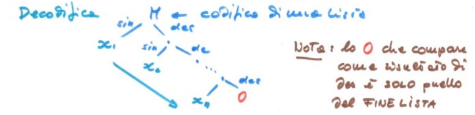
\includegraphics[scale=0.7]{"img/declista.png"}
\end{center}
\end{figure}

\paragraph{Strutture dati derivanti}


Array(lunghezza nota):
\begin{displaymath}
	x_1, \dots, x_n \Rightarrow [x_1, \dots, x_n] = [x_1, \dots, [x_{n-1}, x_n]] \dots ]
\end{displaymath}

Matrici:
\begin{displaymath}
\begin{matrix}
a_{11} & a_{12} \\
a_{21} & a_{22}
\end{matrix}
\Rightarrow
\begin{bmatrix}
a_{11} & a_{12} \\
a_{21} & a_{22}
\end{bmatrix}
\Rightarrow
[[a_{11}, a_{12}], [a_{11}, a_{12}]]
\end{displaymath}

Grafi: utilizzando le liste di adiacenza o le matrici di adiacenza.

\section{Lezione 5}
Sistema di calcolo $\textit{RAM}$: macchina $\textit{RAM}$ + linguaggio $\textit{RAM}$ (assembly semplificato). Consente di definire rigorosamente:
\begin{itemize}
	\item $\textit{PROG} \sim \mathbb{N}$
	\item $C(P, \_) \textit{RAM}(P, \_) $, semantica dei programmi
	\item $F(\textit{RAM})$, potenza computazionale
\end{itemize}

Forse l'idea di potenza computazionale fornita in prima istanza ($F(\textit{RAM})$ è stringente in quando la macchina $\textit{RAM}$ è molto semplice, successivamente introdurremo la macchina $\textit{WHILE}$ (JVM) e comfronteremo le loro potenze computazionali. Se avremo $F(\_)$:
\begin{itemize}
	\item diverse $\Rightarrow$ ciò che è computabile dipende dallo strumento
	\item uguale $\Rightarrow$ computabilità (tesi di Church)? posso calcosare stessi insiemi di funzioni?
\end{itemize}

\paragraph{Sistema di calcolo $\textit{RAM}$}
La macchina $\textit{RAM}$ è composta da:
\begin{itemize}
	\item $L$, program counter, indica indirizzo della prossima istruzione da eseguire;
	\item $P$, programmma, formato da istruzioni;
	\item $R$, memoria, insieme di registri e ogni cella può contenere un numero $\in \mathbb{N}$, dove $R_1$ contiene l'inpur e $R_0$ l'output.
\end{itemize}



La terminazione è data da $L=0$. 



Output: $\phi_P(x)=\textit{contenuto}(R_o)$ o $\perp$ in caso di loop, indichiamo con $\phi_P$ la semantica di $P$.

\paragraph{Linguaggio $\textit{RAM}$}
\begin{itemize}
	\item $R_k \leftarrow R_{k} + 1 $
	\item $R_k \leftarrow R_{k} \dot{-} 1; x \dot{-} y = x-y \textit{ if } x \geq y \textit{ else } 0$
	\item $\textit{if } R_k=0 \textit{ then goto } m; m=\{1, |P| \}; |P|=\textit{numero di istruzioni di } P $
\end{itemize}

\paragraph{Semantica Operazionale}
Ovvero specificare il significato di ogni istruzione, e quindi dei programmi, specificando l'effetto che quell'istruzione ha sui registri della macchina.


Come descrivo l'effetto di un'istruzione? $S$=Stato=foto della macchina. Prendo $S$ prima e dopo l'esecuzione di un'istruzione.
$S_{\textit{init}}, S_1, S_{\textit{fin}}$, $P$ induce una sequenza di stati.



La semantica di $P$:
\begin{displaymath}
	\phi_{P} =
	\begin{cases}
		&y \textit{ se finisce} \\
		&\perp \textit{ altrimenti}
	\end{cases}
\end{displaymath}


\subsection{Ingredienti della definizione formale di semantica}
\paragraph{Stato}
\begin{displaymath}
	\begin{split}
	& S:\{L,R\} \rightarrow \mathbb{N} \\
	& \textit{Stati} = \mathbb{N}^{\{L,R\}} \\
	& S(R_k): \textit{contenuto del registro $R_k$ quando la macchina è nello stato $S$} \\
	& \textit{stato finale}: S(L)=0 \Rightarrow \textbf{HALT} \\
	& \textit{dato}: \mathbb{N} (infatti \textit{DATI} \sim \mathbb{N})
	\end{split}
\end{displaymath}


\paragraph{Inizializzazione}
Dato il dato $n$ prepara la macchina nello stato iniziale:
\begin{itemize}
	\item $S_{\textit{init}}(L)=1$
	\item $S_{\textit{init}}(R_1)=n$
	\item $\forall i \neq 1 : S_{\textit{init}}(R_i)=0$
\end{itemize}

\paragraph{Programmi}
	$PROG=\{\textit{programmi RAM}\}, P \in PROG; |P|= \#\textit{istrizioni}$
	
\paragraph{Esecuzione}
Dinamica del programma $\Rightarrow$ funzione stato prossimo.



$\sigma: \textit{stati} \times \textit{PROG} \rightarrow \textit{stati}_{\perp}$; $\sigma(S,P)=S'$



Lo stato che segue lo stato $S$ dopo l'eesecuzione di un'istruzione di $P$:
\begin{itemize}
	\item dipende dall'istruzione che devo eseguire
	\item l'istruzione dipende da $S(L)$
\end{itemize}

\begin{enumerate}
	\item se $S(L)=0$ allora $S'=\perp$
	\item se $S(L) > |P|$ allora $S'(L)=0$ e $\forall i: S'(R_i)=S(R_i)$
	\item se $1 \leq S(L) \leq |P|$: considero l'istruzione $S(L)-esima$:
		\begin{itemize}
			\item $R_k \leftarrow R_k +/\dot{-}1$:
			\begin{itemize}
				\item $S'(R_k)=S(R_k) +/\dot{-}1$
				\item $S'(L)=S(L)+1$
				\item $\forall i \neq k: S'(R_i)=S(R_i)$
			\end{itemize}
			\item $\textit{if } R_k=0 \textit{ then goto }m$:
			\begin{itemize}
				\item $S'(R_i)=S(R_i)$
				\item $S'(L)=m \textit{ if } S(R_k)==0 \textit{ else } S(L)+1$
				
			\end{itemize}
			
		\end{itemize}
\end{enumerate}
\paragraph{Semantica di $P$}

\begin{displaymath}
	\begin{split}
		&\phi_P:\mathbb{N} \rightarrow \mathbb{N}_{\perp} \\
		&\phi_P(n) = 
		\begin{cases}
			&y \textit{ se } S_m(L)=0 \textit{ e } S_m(R_0)=y \\
			&\perp \textit{se va in loop}
		\end{cases}
	\end{split}
\end{displaymath}
\paragraph{Potenza computazionale di $\textit{RAM}$}
$F(\textit{RAM}=\{f \in \mathbb{N}^{\mathbb{N}}_{\perp}: \exists P \in \textit{PROG}, \phi_P=f\} = \{ \phi_{P}:P \in \textit{PROG} \} \subseteq \mathbb{N}^{\mathbb{N}}_{\perp}$.



Incluso stretto per intuizione.














\section{Lezione 6}
\subsection{$\textit{PROG} \sim \mathbb{N}$ su programmi \textit{RAM}}
\paragraph{Come codificare programmi in numeri e ritorno biunivocamente}
Applichiamo a ogni istruzione del programma un'aritmetizzazione e poi uniamo i vari numeri generati per creare un singolo numero tramite la codifica utilizzata con la lista di numeri + Cantor.
Per il ritorno, sappiamo decodificare la lista finale; se l'aritmetizzazione (\textit{Ar}) è invertibile allora da $n$ posso ricostruire univocamente il sorgente.



Ci MAnca solo il passaggio fatto da \textit{Ar}: da istruzioni a numeri e viceversa. Questo passaggio si dice aritmetizzare o godelizzare.
\subsection{Come aritmetizzare?}
\begin{displaymath}
	\begin{split}
		&\textit{Ar}: \textit{istruzione} \rightarrow \mathbb{N} \textit{ t.c. } \textit{Ar}(\textit{istr}=n) \leftrightarrow \textit{Ar}^{-1}(n)=\textit{istr} \\
		&\textit{Ar}(R_k \leftarrow R_k + 1)=3k \\
		&\textit{Ar}(R_k \leftarrow R_k \dot{-} 1)=3k+1 \\
		&\textit{Ar}(\textit{if }R_k = 0 \textit{ then goto }m =3<k,m>-1 \textit{ come fare +2} 
	\end{split}
\end{displaymath}
\paragraph{Com'è fatto $\textit{Ar}^{-1}$}
Utilizzo il resto della divisione per 3, quindi $||n||_3$ ($n$ modulo 3):
\begin{itemize}
	\item 0: $n=3k \Rightarrow R_{\frac{n}{3}} \leftarrow R_{\frac{n}{3}}+1$;
	\item 1: $n=3k+1 \Rightarrow R_{\frac{n-1}{3}} \leftarrow R_{\frac{n-1}{3}}\dot{-}1$;
	\item 2: $n=<k,m>-1 \Rightarrow <k,m>=\frac{n+1}{3} \Rightarrow \textit{if } R_{\textit{sin}\frac{n+1}{3}} = 0 \textit{ then goto } R_{\textit{des}\frac{n+1}{3}}$.
\end{itemize}
\paragraph{Da programmi a numeri}
$\textit{cod}(P)=<\textit{Ar}(\textit{istr}_1), \dots, \textit{Ar}(\textit{istr}_m)>$
\paragraph{Da numeri a programmi}
Come la decodifica destro/sinistro con le parti sinistra che "subiscono" $\textit{Ar}^{-1}$, anche in questo caso ci fermiamo quando troviamo lo $0$ nel lato destro.
\paragraph{Osservazioni}
\begin{itemize}
	\item i numero diventano linguaggio di programmazione;
	\item potrei scrivere $F(\textit{RAM})= \{\phi_{P}:P \in \textit{PROG}\}$ come $F(\textit{RAM})= \{ \phi_i \}_{i \in \mathbb{N}}$;
	\item per il sistema \textit{RAM} si ha rigorosamente $F(\textit{RAM}) \sim \mathbb{N} \cancel{\sim} \mathbb{N}^{\mathbb{N}}_{\perp}$, quindi alcuni problemi non sono automatizzabili;
	\item forse, cosiderando un sistem adi calcolo $C$ più soffisticato ma comunque rigorosamente trattabile come \textit{RAM}, potremmo dare un'idea formale di "ciò che è calcolabile automaticamente" come $F(C)$ che sia più ampia di $F(\textit{RAM})$;
	\item se dimostriamo  che $F(C)=F(\textit{RAM})$ allora cambiare tecnologia non cambia ciò che è calcolabile $\Rightarrow$ la calcolabilità è intrinseca ai problemi: perchè non catturarla matematicamente? (no macchine, no linguaggio, ...).
\end{itemize}

\subsection{Sistema di calcolo \textit{WHILE}}
Memoria $x_0, \dots, x_20$ con $x_0$ output e $x_1$ input. Le variabili contengono numeri arbitrariamente grandi e di conseguenza in una singola variabile posso salvare, per esempio con Cator, più di un semplice numero.



Non abbiamo un program counter in quanto il linguaggio \textit{WHILE} è strutturato.

\paragraph{Linguaggio \textit{WHILE}}
Sintassi induttiva: ho delle fasi semplici, con passi induttivi faccio cose più complicate.
\begin{itemize}
	\item $[BASE]$: comando assegnamento: $x_k=0$, $x_k=x_j+1$, $x_k=x_j\dot{-}1$; 
	\item $[PASSI]$: comando while: while $x_k \neq 0$ do $C$, con $C$ che può essere:
		\begin{itemize}
			\item comando di assegnamento
			\item comando while
			\item comando composto
		\end{itemize}
	\item $[PASSI]$: comando composto: $\underline{\textit{BEGIN}}$ $ C_1, \dots, C_m $ $\underline{\textit{END}}$, con $C$ come sopra.
\end{itemize}

Possiamo quindi dire che un programma \textit{WHILE} è un comando composto.


$w-\textit{PROG} = \{ \textit{programmi WHILE} \} \leftarrow$ costruiti induttivamente.


Semantica di $w$: $\psi_w:\mathbb{N}\rightarrow\mathbb{N}$


\paragraph{$w-\textit{PROG}$} Per dimostrare una proposizione su $w-\textit{PROG}$:
\begin{enumerate}
	\item dimostro proposizione sugli assegnamenti;
	\item suppongo proposizione su $C$ e la dimostro su $while x_k \neq 0 do C$;
	\item suppongo vera la proposizione su $C_1, \dots, C_m$ e la dimostro su $\underline{\textit{BEGIN}}$ $ C_1, \dots, C_m$ $ \underline{\textit{END}}$.
\end{enumerate}
\subsubsection{Dimostrazioni induttive su alberi bianri}
\begin{center}
\begin{forest}
[$\bullet$
	[$\bullet$
		[$\bullet$]
		[$\bullet$[$\bullet$][$\bullet$]]]
	[$\bullet$]
]
\end{forest}
\end{center}
Dividiamo i nodi in nodi interni e foglie.
\begin{enumerate}
	\item $[BASE]$: $\bullet$ è un albero binario
	\item $[PASSO]$: se $T_1$ e $T_2$ sono alberi binari allora 
	\begin{forest}
[$\bullet$
	[$T_1$]
	[$T_2$]
]
\end{forest}
è un albero binario
\item nient'altro è un albero binario
\end{enumerate}

\paragraph{su ogni albero binario, il numero di nodi interni è minore di 1 rispetto alle foglie = P}
Per induzione:
\begin{enumerate}
	\item $[BASE]$: $\bullet$, 1 foglia e 0 nodi interni $\Rightarrow$ \textbf{VERO}
	\item $[PASSO]$: suppongo vero P su $T_1$ e $T_2$, ovvero suppongo vero:
		\begin{itemize}
			\item $T_1$: foglie $F_1$, nodi interni $F_1-1$
			\item $T_2$: foglie $F_2$, nodi interni $F_2-1$	
		\end{itemize}
\end{enumerate}
Dimostro vero P per:
\begin{forest}
[$\bullet$
	[$T_1$]
	[$T_2$]
]
\end{forest}
ovvero $F_1+F_2$ foglie, e $F_1-1+F_2-1+1=F_1+F_2-1$ nodi interni $\Rightarrow$ \textbf{VERO}

\paragraph{Depth}
\begin{enumerate}
	\item $[BASE]$: $depth(\bullet)= 0$
	\item $[BASE]$: $depth($\begin{forest}
[$\bullet$
	[$T_1$]
	[$T_2$]
]
\end{forest}$)= 1+max(depth(T_1)+depth(T_2))$

\end{enumerate}

\section{Lezione 7}
\subsection{Esecuzione su una macchina WHILE (intuituvamente)}
\begin{enumerate}
	\item inizializzazione: imposto le variabili $x_0, \dots, x_{20}$ come $0,n,0,\dots, 0$;
	\item esecuzione: eseguo le istruzione del programma $w$ (non ho bisogno del program counter);
	\item terminazione: quando le isctruzioni di $w$ terminano oppure ho un loop;
	\item output: contenuto di $x_0$, quindi $\Psi(n)=\textit{cont}(x_0)/\perp$.
\end{enumerate}
\paragraph{Semantica del programma $w$}
$\Psi_w: \mathbb{N} \rightarrow \mathbb{R}_{\perp}$.

\subsection{Definizione formale di semantica di un programma WHILE}
\begin{itemize}

\item Stato: foto della macchina in un tempo $t$ ovvero una tupla/vettore di 21 componenti: $(c_0, \dots, c_{20})$ con $c_i$ contenuto della cella $x_i$.
\begin{displaymath}
	W-\textit{Stati}=\mathbb{N}^{21}, \textit{ stato } \underline{x} \in \mathbb{N}^{21} \textit{ (vettore \underline{$x$})}
\end{displaymath}
\item Dati: $\mathbb{N}$
\item Inizializzazione: $w\textit{-in}: \mathbb{N} \rightarrow \mathbb{N}^{21}$ con $w\textit{-in}(n)=(0,n,0,\dots,0)$
\item Semantica operazione: \begin{displaymath}
		[](): w\textit{-comandi} \times w\textit{-stati} \rightarrow w\textit{-stati}_{\perp} 
		; [C](\underline{x})=\underline{y}
\end{displaymath} 
con $C$ comdando, $\underline{y}$ è lo stato prossimo partendo da $\underline{x}$ eseguendo $C$
\end{itemize}
Posso definire intuitivamente $[C](\underline{x}$ sulla struttura induttiva del comando $C$:
\begin{itemize}
\item $[BASE]$ Assegnamenti:
\begin{displaymath}
	\begin{split}
		&[x_k=0](\underline{x}) = \underline{y} \textbf{ con } y_i=\begin{cases}
				x_i &\textbf{ se } i \neq k \\
				0 &\textbf{ se } i = k
			\end{cases} \\		
		&[x_k=x_j +/\dot{-}1](\underline{x}) = \underline{y} \textbf{ con } y_i=\begin{cases}
				x_i &\textbf{ se } i \neq k \\
				x_j +/\dot{-}1 &\textbf{ se } i = k
			\end{cases} 
	\end{split}
\end{displaymath}
\item $[PASSO]$ Comando composto: $[\underline{\textit{BEGIN}}\textit{ }C_1, \dots, C_m \textit{ } \underline{\textit{END}}]$, conosco $[C_i]$ per ipotesi induttiva, ovvero conosco cosa fa ogni singolo comando.
\begin{displaymath}
	[C_m](\dots(([C_2]([C_1](\underline{x})))\dots) = \underline{y} = [C_1] \cdot \dots \cdot [C_m](\underline{x})
\end{displaymath}
\item $[PASSO]$: Comando while: $[\underline{\textit{WHILE}}\textit{ }x_k \neq 0 \underline{\textit{DO}}\textit{ } C]$, conosco $[C_i]$ come sopra.
\begin{displaymath}
	[C](\dots(([C]([C](\underline{x})))\dots) = \underline{y}
\end{displaymath}
Quante volte applico $C$? Tante volte quanto serve per azzerare $x_k$ dello stato risultante durante l'iterazione del comando $C$ ovvero
\begin{displaymath}
	\begin{cases}
		&[C]^e(\underline{x}) \textbf{ con } e=\mu t(\textit{$k$-esima componente di }[C]^{(t)}(\underline{x})=0 )\\
		&\perp \textit{ altrimenti}
	\end{cases}
\end{displaymath}
dove $\mu t$ è il minor numero di volte.
\end{itemize}

\paragraph{Semantica di $w$ e $w\textit{-prog}$}
$\Psi_w(n)=\textbf{Pr}(0, [w](w\textit{-in}(n))$; proiezione 0-esima ci restituisce l'output applicando $[w]$ allo stato prodotto dall'inizializzazione con $x_1=n$.

\subsection{Potenza computazionale sistema WHILE}
\begin{displaymath}
	F(WHILE)=\{ f \in \mathbb{N}_{\perp}^{\mathbb{N}}: \exists w \in w\textit{-PROG}, f= \Psi_w \} = \{ \Psi_w: w \in w\textit{-PROG} \}
\end{displaymath}
\subsubsection{Relazione tra $F(RAM)$ e $F(WHILE)$?}
Che relazione esiste tra $F(WHILE$ e $F(RAM)=\{ \phi_P:P \in \textit{PROG} \} $?
\begin{itemize}
	\item $F(RAM) \subsetneq F(WHILE)$, sarebbe anche comprensibile vista la semplicità della macchina $RAM$;
	\item Insiemi con intersezioni o disgiunti, sarebbe preoccupante perchè il concetto di calcolabile dipenderebbe dalla macchina;
	\item $F(WHILE) \subsetneq F(RAM)$, sarebbe sorprendente poichè $WHILE$ sembra più soffisticata di $RAM$;
	\item $F(RAM) = F(WHILE) \Rightarrow$ calcolabile non dipende dalla tecnologia
\end{itemize}
\subsubsection{Confronto tra due sistemi di calcolo}
Poniamo di avere due sistemi di calcolo $C_1$ e $C_2$ con i relativi programmi $C_1\textit{-PROG}$ e $C_2\textit{-PROG}$. 
\begin{displaymath}
	\begin{split}
		& F(C_1) = \{ f \in \mathbb{N}_{\perp}^{\mathbb{N}}: f= \Psi_{P_1} \textit{ per qualche $P_1$ e $C_1$}-PROG \} = \{ \Psi_{P_1} : P_1 \in C_1\textit{-PROG} \} \\
		& F(C_2) = \{ f \in \mathbb{N}_{\perp}^{\mathbb{N}}: f= \phi_{P_2} \textit{ per qualche $P_2$ e $C_2$}-PROG \} = \{ \phi_{P_2} : P_2 \in C_2\textit{-PROG} \} \\
	\end{split}
\end{displaymath}
Come mostriamo che $F(C_1) \subseteq F(C_2)$ ovvero che il primo non supera il secondo? Dimostro che 
\begin{displaymath}
	\forall f \in F(C_1) \Rightarrow f \in F(C_2)
\end{displaymath}
ovvero che per ogni elemento del primo insieme allora è anche nel secondo insieme (dimostrazione di inclusione).



Risolviamo questo problema con un traduttore, prende un programma in un linguaggio e lo traduce in un altro linguaggio; per esempio quando compilo un programma in $C++$ creo un assembly, questo implica che $C++$ è al più potente come assembly. Matematicamente possiamo descrivere un traduttore come 
\begin{displaymath}
	\exists P_1 \in C_1 \textit{-PROG}: f=\Psi_{P_1} \Rightarrow \exists P_2 \in C_2\textit{-PROG}: f=\Phi_{P_2},
\end{displaymath}
per ogni programma nel primo sistema ne esiste uno equivalente a un programma del secondo sistema.


\subsection{Concetto di traduttore}
Dati i sistemi $C_1$ e $C_2$, una traduzione da $C_1$ a $C_2$ è una funzione $T: C_1\textit{-PROG} \rightarrow C_2\textit{-PROG}$ con le seguenti proprietà:
\begin{itemize}
	\item $[\underline{Programmabile}]$: è programabbile;
	\item $[\underline{Completa}]$: traduce ogni $C_1\textit{-PROG}$ in $C_2\textit{-PROG}$;
	\item $[\underline{Corretta}]$: mantiene la semantica $\forall P \in C_1\textit{-PROG}: \phi_{T(P)}=\Psi_P$, è la formalizzazione del concetto di compilatore (nota che $\phi_{T(P)}$ è l'oggetto e $Psi_P$ il sorgente).
\end{itemize}
Se esiste $T: C_1\textit{-PROG} \rightarrow C_2\textit{-PROG}$ allora $F(C_1) \subseteq F(C_2)$. Dimostrazione:
\begin{displaymath}
	\begin{split}
		&f \in F(C_1) \Rightarrow \exists P \in C_1\textit{-PROG}: f= \Psi_p \\
		&\textit{a $P$ applico T, ottengo}\\
		&T(P) \in C_2\textit{-PROG} \textit{ (completezza), con } \phi_{T(P)} = \Psi_P = f \textit{ (correttezza)} \\
		&\textit{esiste dunque un PROG in $C_2\textit{-PROG}$ per $f$, per cui }f \in F(C_2).
	\end{split}
\end{displaymath}


\section{Lezione 8}
Mostreremo $F(WHILE) \subseteq F(RAM)$, mostreremo una traduzione $comp:W-PROG \rightarrow PROG$. Per comodità utilizzeremo il linguaggio RAM etichettato: etichetto una riga (istruzione) per fare un salto, ovviamente ho la stessa potenza computazionale di RAM.



In quanto $W-PROG$ è definito induttivamente $comp$ può essere definito induttivamente:
\begin{enumerate}
	\item $[BASE]$ mostro come compilare gli assegnamenti;
	\item $[PASSO]$ per ipotesi induttiva assumo dato $comp(C_1), \dots, comp(C_m)$ e mostro come compilare il comando composto $\underline{BEGIN} \textit{ } C_1, \dots, C_m \textit{ } \underline{END}$;
	\item $[PASSO]$ per ipotesi induttiva assumo dato $comp(C)$ e mostro come compilare il comando while $\underline{WHILE}\textit{ } X_k \neq 0\textit{ } \underline{DO}\textit{ } C$.
\end{enumerate}

\subsection{Costruzione induttiva di $comp$}
In generale tradurremo $X_k$ con $R_k$ ovvero variabili di WHILE in registri RAM ($21 \Rightarrow \infty$).
\paragraph{$[BASE]$ assegnamenti}
\begin{itemize}
	\item $comp(X_k := 0)$
	\begin{displaymath}
		\begin{split}
			 \underline{loop}: &\text{ } if \text{ } R_k == 0 \textit{ then goto \underline{exit}} \\
			 & R_k \leftarrow R_k \dot{-} 1 \\
			 & if \text{ } R_{21} == 0 \textit{ then goto \underline{loop}} \\
			 \underline{exit}: & R_k \leftarrow R_k \dot{-} 1 
		\end{split}
	\end{displaymath}
	Uso $R_{21}$ perchè sarà sempre uguale a 0, WHILE ha 21 variabili (da 0 a 20).
	\item $comp(X_k := X_j +/\dot{-} 1)$
	\begin{itemize}
		\item se $k==j$: $R_k \leftarrow R_k +/\dot{-} 1$
		\item altrimenti: \begin{enumerate}
			\item salvo $X_j$ in $R_{22}$;
			\item azzero $R_k$;
			\item metto in $R_j$ e $R_k$ il contenuto di $R_22$ (un ciclo che fa + 1 al $R_{22}$ e somma 1 a a $R_k$ e $R_k$;
			\item sommo/sottraggo 1 a $R_k$.
		\end{enumerate}
	\end{itemize}
\end{itemize}
\paragraph{$[PASSO]$}
\begin{itemize}
	\item comando composto: basta prendere la sequenza di comando e creare la sequenza di compilazione dei comandi
	\item comando while: $comp(\underline{while}\text{ } x_k \neq 0 \textit{ \underline{do} } C)$:
	\begin{displaymath}
		\begin{split}
			\underline{loop}: &\text{ } if \text{ } R_k == 0 \textit{ then goto \underline{exit}} \\
			 & comp(C) \\
			 & if \text{ } R_{21} == 0 \textit{ then goto \underline{loop}} \\
			 \underline{exit}: & R_k \leftarrow R_k \dot{-} 1
		\end{split}
	\end{displaymath}
\end{itemize}

\paragraph{Considerazioni}
\begin{enumerate}
	\item il compilatore è facilmente programmabile;
	\item compila ogni sorgente while $\Rightarrow$ completo;
	\item mantiene la semantica: $\Psi_w = \Phi_{comp(w)}  \Rightarrow$ corretto;
\end{enumerate}
quindi $F(WHILE) \subseteq F(RAM)$.

\subsection{$F(RAM) \subseteq F(WHILE)$}
Faremo un interprete (compila riga per riga e ha come output l'output del programma), $I_w$: interprete scritto in WHILE di programmi scritti in RAM.
\begin{itemize}
	\item input di $I_w$: $P \in PROG$ e $x \in \mathbb{N}$, output: $\Phi_P(x)$
	\item input di $I_w$: $codifica(P) = n$ e $x \in \mathbb{N}$, output: $\Phi_n(x) = \Phi_P(x)$
	\item input di $I_w$: $ <x,n>$ con $x$ il dato di input e $n$ la codifica del programma, output: $\Phi_n(x) =\Phi_P(x)$
\end{itemize}
La semantica di $I_w$: $\forall x,n \in \mathbb{N}: \Psi_{I_w}(<x,n>)=\Phi_n(x)=\Phi_P(x)$.
\paragraph{Macro while}
Per comodità, nella scrittura di $I_w$ utilizzeremo un WHILE che ingloba alcune macro che possono essere tradotte in WHILE puro.
\section{Lezione 9}
\subsection{Interprete WHILE di programmi RAM}
\subsubsection{Variabili}
$I_w$ ricrea nelle sue variabili l'ambiente (macchina RAM) in cui esegue $P$.
Se $cod(P)=n$ allora $P$ non userà mai $R_j$ con $j>n$. Posso quindi restringermi a modellare la sequenza $R_0,\dots,R_{n+2}$. Il contenuto della memoria in cui si esegue $P$ può essere considerato in una sola variabile contenente $<a_0,a_1, \dots, a_{n+2}>$.



\noindent
Avremo quindi la seguente configurazione:
\begin{itemize}
	\item $X_0 \Leftarrow <R_0,\dots,R_{n+2}>$;
	\item $X_1 \Leftarrow L$ con $L$ program counter;
	\item $X_2 \Leftarrow x$ ovvero il dato di input;
	\item $X_3 \Leftarrow n$ ovvero il "listato" del programma $P$; 
	\item $X_4 \Leftarrow$  codice dell'istruzione da eseguire prelevata da $X_3$ nella posizione $X_1$. 
\end{itemize}

\paragraph{Inizializzazione}
\begin{enumerate}
	\item $X_1 \Leftarrow input(<x,n>)$
	\item $X_2:= sin(X_1)$ ovvero il dato di input;
	\item $X_3:= sin(X_1)$ ovvero il "listato" del programma $P$; 
	\item $X_1 :=1$. 
\end{enumerate}
\subsubsection{Codice interprete in macrowhile}
\begin{algorithm}
        \begin{algorithmic}[1]
        		\While{$(X_1 \neq 0)$}\Comment{HALT con $L=0$}
        		\If{$(X_1 > length(X_2))$} $X_1:=0$ \Comment{Ho finito le istrizioni}
        		\Else
        			\State $X_4 := Pro(X_1,X_3)$ \Comment{Prendo elemento in pos $X_1$ di $X_3$ (fetch)}
				\If{$(X_4 mod 3 == 0)$} \Comment{$R_k \leftarrow R_k+1$}
					\State $X_5 := X_4/3$
					\State $X_0:= incr(X_5,X_0)$ \Comment{Increm di 1 elem in pos $X_5$ di $X_0$}
					\State $X_1:=X_1+1$ \Comment{Incremento program counter}
            		\EndIf
            		
            		\If{$(X_4 mod 3 == 1)$} \Comment{$R_k \leftarrow R_k\dot{-}1$}
					\State $X_5 := (X_4-1)/3$
					\State $X_0:= decr(X_5,X_0)$ 
					\State $X_1:=X_1+1$ 
            		\EndIf
            		
            		\If{$(X_4 mod 3 == 2)$} \Comment{$\textit{if }R_k==0\textit{ then goto }m$}
					\State $X_5 := sin((X_4+1)/3)$\Comment{$k$}
					\State $X_6 := des((X_4+1)/3)$\Comment{$m$}
					\If{$(Pro(X_5,X_0)==0)$}
						\State $X_1=X_6$
					\Else 
						\State $X_1:=X_1+1$ 
					\EndIf
            		\EndIf
            \EndIf
            \EndWhile
            \State $X_0:=sin(X_0)$
        \end{algorithmic}
    \end{algorithm}

\subsubsection{Conseguenze}
Posso costruire $Comp:PROG\rightarrow W-PROG$:
\begin{itemize}
	\item $n=cod(P)$
	\item $X_1 := <x,n>$
	\item $I_w$
\end{itemize}
Programmabile, completo e corretto.




$\Psi_{comp(P)}(x)=\Psi_{I_w}(<x,n>)=\Phi_n(x)=\Phi_P(x)$ OK!
\paragraph{Teorema di Bohm-Jacopini} Per ogni programma con goto (RAM) ne esiste uno equivalente in linguaggio strutturato (WHILE).

\paragraph{Finalmente..}
$\mathbb{N}_{\perp}^{\mathbb{N}} \bar{\sim} \mathbb{N} \sim PROG \sim F(RAM) = F(WHILE)$
\begin{itemize}
	\item nei sistemi di programmazione RAM e WHILE esistono funzioni non computabili, dimostrato formalmente;
	\item i sistemi RAM e WHILE, pur profondamente diversi, calcolano le stesse cose.
\end{itemize}




Usiamo $comp:W-PROG \rightarrow PROG$ sse $I_w(\Psi_{I_w}(<x,n>)=\Phi_n(x))$.

\begin{displaymath}
	\begin{split}
		&U=comp(I_w) \in PROG \\
		\Phi_U(<x,n>)=\Psi_{I_w}(<x,n>)=\Phi_n(x)
	\end{split}
\end{displaymath}
Nel sistema di programmazione RAM esiste un programma RAM capace di simulare qualunque altro programma RAM! $U$ è detto interprete universale (RAM).

\subsubsection{Riflessioni concetto di calcolabilità}
Due sistemi profondamente diversi che determinano la stessa idea di calcolabilità. Possiamo sublimare il concetto di calcolabile?



Possiamo pensare di definire ciò che è calcolabile a prescindere dalle macchine che usiamo per calcolare?



Possiamo pensare di definire ciò che è calcolabile in termini più astratti, matematici, "lontani dall'informatica"?


\section{Lezione 10}
\subsection{Chiusura di insiemi rispetto ad operazioni}
Dato un insieme $U$, si definisce un'operazione su $U$ una qualunque funzione $op:U\times \dots \times U \rightarrow U$ con $U$ ripetuta $k$ volte in input: $k$=arietà dell'operazione.
\paragraph{Esempi} $U=\mathbb{N}$
\begin{itemize}
	\item $+:\mathbb{N} \times \mathbb{N} \rightarrow \mathbb{N}$, somma: $+(5,3)=8$, operazione binaria;
	\item $\lfloor \sqrt{} : \mathbb{N} \rightarrow \mathbb{N}$, radice troncata, operazione unaria;
	\item $Pro_t^n: \mathbb{N} \times \dots \times \mathbb{N} \rightarrow \mathbb{N}$ con $n$ volte in input, proiezione $t$-esima, operazione $n$-aria.
\end{itemize}
\subsubsection{Chiusura}
L'insieme $a \subseteq U$ è \underline{chiuso} risetto all'operazione $op:U^k \rightarrow U$ sse $\forall a_1, \dots, a_k \in A: op(a_1, \dots, a_k) \in A$, ovvero l'operazione non mi "amplia" $A$.
\paragraph{Esempi}
\begin{itemize}
	\item $+: \mathbb{N}^2 \rightarrow \mathbb{N}, PARI \subseteq \mathbb{N}$. $PARI$ è chiuso per $+$? si, $2k + 2j =2(k+j)$
	\item $+: \mathbb{N}^2 \rightarrow \mathbb{N}, DISPARI \subseteq \mathbb{N}$. $DISPARI$ è chiuso per $+$? no, $23+3=6$
	\item $/: \mathbb{Q}^2 \rightarrow \mathbb{Q}, \mathbb{N} \subseteq \mathbb{Q}$. $\mathbb{N}$ è chiuso per $/$? no, $5/2 \bar(\in) \mathbb{N}$
\end{itemize}
Per rispondere si dobbiamo dimostrare che vale, nel nostro caso, per ogni coppia; per rispondere no basta un controesempio.




In generale: se $\Omega$ è un'insieme di operazioni su $U$, allora $A \subseteq U$ è chiuso rispetto a $\Omega$ se è chiuso per ogni operazione in $\Omega$.
\paragraph{Esempi}
\begin{itemize}
	\item $\Omega = \{ +, - \}, PARI \subseteq \mathbb{N} \rightarrow$ somma si, prodotto si ($2k \cdot 2j = 4kj$);
	\item $\Omega = \{ +, - \}, DISPARI \subseteq \mathbb{N} \rightarrow$ somma no, prodotto si ( $(2k+1)  (2j+1) = 4kj+2k+2j+1$ è dispari).
\end{itemize}
\subsubsection{Chiusura di un'insieme}
\paragraph{Problema:} Sia $A \subseteq U$ e $op:U^k \rightarrow U$. Qual è il più piccolo sottoinsieme di $U$ che \underline{contiente $A$} e \underline{sia chiuso per $op$}? In pratica voglio allargare $A$ per renderlo chiuso.
\paragraph{Risposte ovvie:}
\begin{itemize}
	\item se $A$ è chiuso per $op$ allora $A$ stesso;
	\item sicuramente $U$ soddisfa le due richieste ma non è sempre il più piccolo.
\end{itemize}
\paragraph{Esempio} Sia $A=\{2,3\} \subseteq \mathbb{N}$ e $+:\mathbb{N}^2 \rightarrow \mathbb{N}$, qual è il più piccolo insieme che soddisfa le proprietà sopra? Sicuramente $\mathbb{N}$ ma non è il più piccolo:sicuramente non ci servono 0 e 1. Non basta nemmeno aggiungere $\{ 4,5,6 \}$ perchè devo soddisfare la chiusura anche sui valori che aggiungo all'insieme che sto cercando.



\paragraph{Teorema:} Sia $A \subseteq U$ e $op:U^k \rightarrow U$. Il più piccolo sottoinsieme di $U$ contenente A è chiuso rispetto a $op$ si ottienecalcolando la chiusura rispetto a $op$, cioè l'insieme $A^{op}$ definito induttivamente come:
\begin{enumerate}
	\item $\forall a \in A \Rightarrow a \in A^{op}$;
	\item $\forall a_1, \dots, a_k \in A^{op} \Rightarrow op(a_1, \dots, a_k) \in A^{op}$;
	\item nient'altro sta in $A^{op}$.
\end{enumerate}
Possiamo dare la seguente definizione più operativa:
\begin{enumerate}
	\item metti in $A^{op}$ tutti gli element di $A$;
	\item applica $op$ a una $k$-tupla di elementi in $A^{op}$;
	\item aggiungo il riultato in $A^{op}$ se non è già presente;
	\item reitero i punti 2 e 3 finche $A^{op}$ cresce;
	\item output $A^{op}$.
\end{enumerate}

\paragraph{Esempio}
$A=\{2,3\}, A \subseteq \mathbb{N}$ e voglio trovare $A^+$:
\begin{enumerate}
	\item $A^+ \leftarrow A$;
	\item $2+3=5 \cancel{\in} A^+ \Rightarrow A^+=\{2,3,5\}$;
	\item $2+2,3+3, 5+5, \dots \cancel{\in} A^+ \Rightarrow A^+=\{2,3,4,5,6,10, \dots \}$;
	\item $\dots$.
	\item output: $A^+ = \mathbb{N} \backslash \{0,1\}$.
\end{enumerate}

\subsubsection{Chiusura di un insieme rispetto a un insieme di operazioni}
$A^\Omega$ si ottiene generalizzando il processo per un'operazione induttivamente:
\begin{enumerate}
	\item $\forall a \in A \Rightarrow a \in A^{\Omega}$;
	\item $\forall i \in \{ 1,\dots,t \} \forall a_1, \dots, a_k \in A^{\Omega} \Rightarrow op_i(a_1, \dots, a_k) \in A^{\Omega}$;
	\item nient'altro sta in $A^{\Omega}$.
\end{enumerate}

\subsubsection{Verso una definizione teorica di calcolabilità}
\paragraph{Astratta}: che astraeda qualunque connotato informatico;




\paragraph{Roadmap}:
\begin{enumerate}

	\item $ELEM$: insieme di funzioni che qualunque idea di calcolabile si voglia proporre deve considerare calcolabili; $ELE$ non può esaurire il concetto di calcolabilità $\Rightarrow$ ampliare;
	\item $\Omega$: insieme di operazioni su funzioni che costruiscono funzioni. Le $op$ in $\Omega$ sono banalmente implementabili $\Rightarrow$ se le applico a funzioni calcolabili ottengo nuove funzioni calcolabili;
	\item $ELEM^\Omega = P =$ classe delle funzioni ricorsive parziali. $P \rightarrow$ la nostra idea astratta della classe delle funzioni calcolabili.


\end{enumerate}
	
\section{Lezione 11}

\subsection{$ELEM$: nucleo delle funzioni calcolabili}
$ELEM=$
\begin{displaymath}
\begin{split}
	\{ successore:&S(x)=x+1, x \in \mathbb{N} \\
	zero:&O^n(x_1,\dots, x_n)=0, x \in \mathbb{N}, \textit{ //prende $n$ input e restituisce 0} \\
	proiettori:&Pro^n_k(x_1,\dots, x_n)=x_k, x \in \mathbb{N} \}\end{split}
\end{displaymath}
Queste funzioni sono facilmente implementabili e sicuramente calcolabili.



Ovviamente $ELEM$ non può essere considerato come l'idea teorica di tutto ciò che è calcolabile, per esempio $f(x)=x+2 \cancel{\in} ELEM$ ma $f$ deve essere considerata calcolabile!



$\Rightarrow$ $ELEM$ deve essere ampliata mantenendo l'idea di induttivamente calcolabile.

\subsection{Operatore di composizione di funzioni}
Sia $h:\mathbb{N}^k \rightarrow \mathbb{N}$ e $g_1, \dots, g_k: \mathbb{N}^k \rightarrow \mathbb{N}$, denoteremo $\underline{x} \in \mathbb{N}^k$.
\begin{displaymath}
	\begin{split}
		&COMP(h, g_1, \dots, g_k): \mathbb{N}^k \rightarrow \mathbb{N} \textit{ definito come } \\
		& COMP(h, g_1, \dots, g_k)(\underline{x})=h(g_1(\underline{x}), \dots, g_k(\underline{x})
	\end{split}
\end{displaymath}
Intuitivamente $COMP$ è implementabile, per cui la composizione di "cose" programmabili rimane programmabile.

\subsubsection{Ampliamo $ELEM$ chiudendo rispetto a $COMP$}
$ELEM^{COMP}$ effettivamente amplia $ELEM$ infatti
\begin{displaymath}
	\begin{split}
		&f(x)=x+2 \cancel{\in} ELEM \textit{ ma } f(x) \in ELEM^{COMP} \\
		& \textit{infatti } f(x)=COMP(SUCC,SUCC)(x)=SUCC(SUCC(x)) = f(x)
	\end{split}
\end{displaymath}

$ELEM^{COMP}$ può incarnare teoricamente l'idea di classe delle funzioni calcolabili? \underline{\textbf{NO!}}

\subsection{Operatore di ricorsione primitiva}
\paragraph{Esempio} Fattoriale:
\begin{displaymath}
	FATT(n)=	
	\begin{cases}
		1 &\textit{ se } n = 0 \\
		n(FATT(n-1)) &\textit{ se } n > 0
	\end{cases}
\end{displaymath}

Siano $g:\mathbb{N}^n \rightarrow \mathbb{N}$ e $ h:\mathbb{N}^{n+2} \rightarrow \mathbb{N} $; $g(\underline{x})$ e $h(z,y,\underline{x})$ con $x \in \mathbb{N}^n$
\begin{displaymath}
	RP(h,y)=	f(\underline{x},y)=
	\begin{cases}
		y(\underline{x}) & \textit{ se } y=0 \\
		h(f(\underline{x}, y-1)) & \textit{ se } y>0 
	\end{cases}
\end{displaymath}

\subsubsection{Ampliamo $ELEM^{COMP}$ chiudendo rispetto a $RP$}
$ELEM^{COMP,RP}=\underline{RICPRIM}=$ {funzioni ricorsive privitive}
\begin{displaymath}
	SOMMA(x,y)=
	\begin{cases}
		x=Pro_1^2 &\textit{ se } y=0  \textit{ //non ho costante $x$ in $ELEM$} \\
		SUCC(SOMMA(x,y-1)) &\textit{ se } y>0
	\end{cases}
\end{displaymath}

\begin{displaymath}
	PROD(x,y)=
	\begin{cases}
		0=O^2(x,y) &\textit{ se } y=0  \\
		SOMMA(x,PROD(x,y-1)) \textit{ se } y>0
	\end{cases}
\end{displaymath}

\begin{displaymath}
	PRED(x)=
	\begin{cases}
		0 &\textit{ se } x=0  \\
		x \dot{-} 1 \textit{ se } y>0
	\end{cases}
\end{displaymath}
con il predecessore posso definire la differenza come
\begin{displaymath}
	DIFF(x,y)=
	\begin{cases}
		x &\textit{ se } y=0  \\
		DIFF(PRED(x),y-1) &\textit{ se } y>0
	\end{cases}
\end{displaymath}

\subsection{$RICPRIM$ vs $WHILE$}
$RICPRIM$ contiene già molte funzioni e potrei già chiedermi se ho raggiunto $F(WHILE)$. Mostreremo $RICPRIM \subseteq f(WHILE)$ per induzione strutturare. ($F(WHILE)$ ha possibilità di indefinito mentre $RICPRIM$ no).

\subsubsection{Road map}
\begin{enumerate}
	\item $[BASE]$ le funzioni in $ELEM$ sono in $RICPRIM$;
	\item $[PASSO$ $INDUTTIVO]$ se $h,g_1,\dots,f_k \in RICPRIM \Rightarrow COMP(h,g_1,\dots,g_k \in RICPRIM$;
	\item $[PASSO$ $INDUTTIVO]$ se $g,k \in RICPRIM \Rightarrow RP(g,h) \in RICPRIM$;
	\item null'altro è in $RICPRIM$;
\end{enumerate}
quindi:
\begin{enumerate}
	\item dimostro che $ELEM \subseteq F(WHILE)$;
	\item assumo per ipotesi induttiva che $h,g_1,\dots, g_k \in RICPRIM$ siano in $F(WHILE)$ e dimostro che $COMP(h,g_1,\dots,g_k \in F(WHILE)$;
	\item assumo per ipotesi induttiva che $g,h \in RICPRIM$ siano in $F(WHILE)$ e dimostro che $RP(g,h) \in F(WHILE)$
	
\end{enumerate}
$\Rightarrow RICPRIM \subseteq F(WHILE)$.
\subsubsection{Dimostrazione induttiva}
\begin{itemize}
	\item $[BASE]$: $ELEM \subseteq F(WHILE)$, ovvio (le 3 funzioni iniziali;
	\item $[PASSI$ $INDUTTIVI]$:
		\begin{itemize}
			\item $COMP$: assumiamo per ipotesi induttiva $h,g_1,\dots,g_k \in RICPRIM$ siano in $F(WHILE) \Rightarrow$ esistono $H,G_1,\dots,G_k \in W-PROG$ t.c. $\Psi_H=h,\Psi_{G_1}=g_1,\dots$. Mostro quindi un programma $WHILE$ che calcola $COMP(h,g_1,\dots,g_k)=h(g_1(\underline{x}),\dots,g_k(\underline{x}))$.
			\begin{algorithm}
			\caption{$w \equiv$}
        \begin{algorithmic}[1]
        		 \State $\underline{BEGIN}$ \Comment{$x_1 \leftarrow \underline{x}$ come $<a_1,\dots, a_n>$}
        		 \State $x_0 := G_1(x_1)$
        		 \State $x_0 := [x_0, G_2(x_1)$] \Comment{calcolo i vari $G$ e poi metto insieme in $H$}
        		 \State $\dots$
        		 \State $x_0 := [x_0,G_k(x_1)]$ \Comment{$x_0 := [G_1(\underline{x}),\dots, G_k(\underline{x})]$}
        		 \State $x_0 := H(x_0)$ \Comment{$x_0:=H(G_1(\underline{x}),\dots,G_k(\underline{x}))$}
        		 \State $\underline{END}$
        		 
        \end{algorithmic}
    \end{algorithm}
    \\
    		quindi $Psi_w(\underline{x})=COMP(h,g_1,\dots,g_k)(\underline{x})$
    			
    			\item $RP$: assumo per ipotesi induttiva $g(\underline{x}), h(z,y,\underline{x}) \in RICPRIM$ in $F(WHILE) \Rightarrow$ esistono $G,H \in W-PROG$ con $\Psi_G=g$ e $\Psi_H=h$.Mostro qundi un programma $WHILE$ che calcola
    			\begin{displaymath}
    				RP(g,h)=f(\underline{x},y)=
    				\begin{cases}
    					g(\underline{x}) &\textit{ se } y=0\\
    					h(f(\underline{x},y-1),y-1,\underline{x}) &\textit{ se } y>0
    				\end{cases}
    			\end{displaymath}
    			
    			Notiamo che $f(\underline{x},2)=h(h(g(\underline{x}),0),1,\underline{x})$
    			\begin{algorithm}
			\caption{$w \equiv$}
        \begin{algorithmic}[1]
        		 \State $\underline{BEGIN}$ \Comment{$x_1 \leftarrow <\underline{x},y>$}
        		 \State $t:=G(\underline{x})$
        		 \State $k:=1$
        		 \While{$k\leq y$}
        		 	\State $t:=H(t,k-1,\underline{x})$
        		 	\State $k:=k+1$
        		 \EndWhile
        		 \State $\underline{END}$
        		 
        \end{algorithmic}
    \end{algorithm}
    \\
    			quindi $\Psi_w(<\underline{x},y>)=RP(g,h)(\underline{x},y)$
    			
		\end{itemize}
	
	
\end{itemize}
Quindi abbiamo dimostrato per induzione strutturale che $RICPRIM \subseteq F(WHILE)$.
\subsubsection{Considerazioni su $RICPRIM$}
\begin{itemize}
	\item vorremo che la nostra "idea teorica" ($RICPRIM$) di calcolabilità raggiungesse almeno quella pratica ($F(WHILE)$), quindi la normale domanda è: l'inclusione è propria? (ovvero inclusione stretta);
	\item è facile dimostrare per induzione strutturale che tutte le funzioni in $RICPRIM$ sono totali (ovvero che terminano sempre);
	\item $F(WHILE)$ continene anche funzioni parziali (programmi infiniti) $\Rightarrow RICPRIM \subsetneq F(WHILE)$;
	\item posso tradurre il $WHILE$ di prima in un $FOR$, $F(FOR)=RICPRIM$;
	\item poniamo di usare $WHILE-LOOP$ che non vanno all'$\infty$, consideramo cioè l'insieme $\tilde{F}(WHILE)=\{ \Psi_w:w \in w-PROG$ e $\Psi_w$ è totale $ \}$;
	\item l'inclusione $RICPRIM=F(FOR) \subseteq \tilde{F}(WHILE)$ è propria? Per diagonalizzazione $RICPRIM \subsetneq \tilde{F}(WHILE)$. In particolare per la funzione di Ackermann:
	\begin{displaymath}
	A(m,n)=
		\begin{cases}
			n+1 &\textit{ se } m=0 \\
			A(m-1,1) &\textit{ se } m>0,n=0 \\
			A(m-1,f(m,n-1)) &\textit{ se } m>0, n>0
		\end{cases}
\end{displaymath}		
	
	 cresce troppo in fretta per essere in $RICPRIM \Rightarrow$ Ackermann $\in \tilde{F}(WHILE)$ ma $\cancel{\in} RICPRIM$ perchè for non può cambiare il "TO $y$", ovvero non può prevedere le iterazioni.
\end{itemize}

\section{Lezione 12}


\end{document}
